\scanpage{162}
% archive foliation: 161
Soit $f:X-Y$ un morphisme \inserted{propre} dominant, $Y$ \inserted{loc. noeth.} \uline{normal} \uline{connexe}.
Alors $\pi_1(X)\to\pi_1(Y)$ a un conoyau fini
(regardons le pt générique $\eta$ de $Y$, et sachant que $\pi_1(\eta)\to\pi_1(Y)$ est surjectif, on est ramené au cas où $Y=\operatorname{Spec}(K)$.
On voit de $=$ qu'on peut supposer $X$ séparable sur $\unsure{k|K}$ et abs\textsuperscript{t} connexe
[remplacer $K$ par une extension \inserted{séparable} finie convenable $K'$], et diviser $\mathcal O_{X'}$ par ses élts nilpotents, \unsure{enfin} prendre une composante connexe de $X'$].
Mais alors $\pi_1(X)\longrightarrow\pi_1(Y)$ est \uline{surjectif}.

\figure{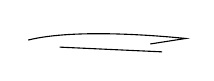
\begin{tikzpicture}[x=1cm,y=1cm]
\draw (0,0) .. controls (.6,.15) and (1.7,.05) .. (2,.02) -- (1.55,-.05);
\draw (.4,-.09) -- (1.7,-.15);
\end{tikzpicture}}

N.B. Si $Y$ n'est pas \uline{normal}, le th. est faux, $=$ si p.ex $X$ est la normalisée de $Y$.
Ex. $Y$ courbe int. sur $k$ alg. clos, avec pt double ordinaire, $X'$ sa normalisée.
On a $\pi_1(\unsure{Y'|X'})=0$, $\pi_1(Y)=\widehat{\mathbb Z}$
\unsure{prouvé} \unsure{en} \deleted{\unsure{se}} par \unsure{comparaison}.

\figure{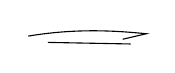
\begin{tikzpicture}[x=1cm,y=1cm]
\draw (0,0) .. controls (.6,.1) and (1.1,.07) .. (1.5,.03) -- (1.2,-.04);
\draw (.25,-.08) -- (1.3,-.1);
\end{tikzpicture}}

On voit facilement que dans le dernier exemple, on ne peut former $\underline{\operatorname{Hom}}_Y(X,Y\amalg Y)$
[car en un \inserted{certain} pt $y_0$ de $Y$, il y a deux pts géométriques dans l'image inverse, alors qu'il n'y en a qu'un au voisinage].
\uline{Supposons cependant} $f:X\to Y$ \uline{universellement ouvert} [p. ex. $Y$ normale], je crois que
